\begin{ex}
 (Ufes) Um avião possui 120 poltronas de passageiros distribuídas em 20 filas. Cada fila tem 3 poltronas do lado esquerdo (denotadas A, B, C) e 3 do lado direito (denotadas D, E, F), separadas pelo corredor do avião. Considere que duas poltronas são vizinhas quando elas estão numa mesma fila e não há poltronas entre elas (observe, portanto, que as poltronas de letras C e D não são consideradas vizinhas).
  \begin{center}
    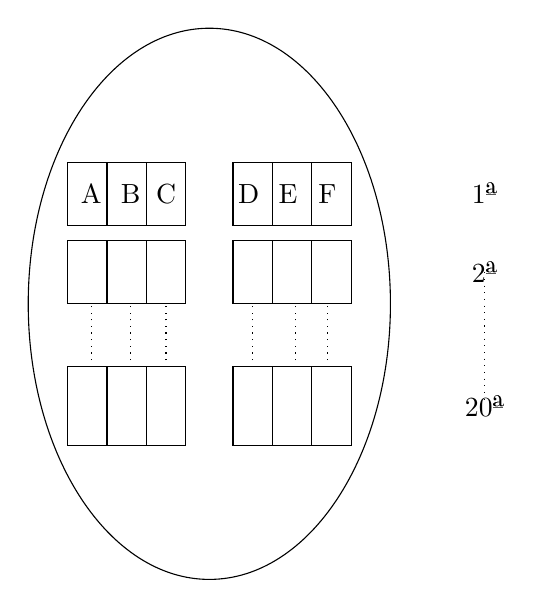
\begin{tikzpicture}
    \draw (-1.8,1) rectangle (-.3,1.8);
    \draw (.3,1) rectangle (1.8,1.8);
    \draw (-1.3,1)--(-1.3,1.8);\draw(-.8,1)--(-.8,1.8);\draw (-1.8,0)rectangle(-.3,.8);
    \draw (.8,1)--(.8,1.8);\draw (1.3,1)--(1.3,1.8);\draw (.3,0) rectangle (1.8,.8);\draw (.8,0)--(.8,.8); \draw (1.3,0)--(1.3,.8);\draw (-1.8,-1.8)rectangle(-.3,-.8);\draw (-1.3,-1.8)--(-1.3,-.8); \draw(-.8,-1.8)--(-.8,-.8);
    \draw (0,0) ellipse (2.3cm and 3.5cm);
    \draw (-1.3,0)--(-1.3,.8);\draw (-.8,0)--(-.8,.8); \draw (.3,-1.8) rectangle (1.8,-.8);\draw (.8,-1.8)--(.8,-.8); \draw (1.3,-1.8)--(1.3,-.8);\draw [dotted] (-1.5,-.8)--(-1.5,0);\draw [dotted] (-1,-.8)--(-1,0);
    \draw [dotted] (-.55,-.8)--(-.55,0); \draw [dotted] (.55,-.8)--(.55,0); \draw [dotted] (1.1,-.8)--(1.1,0);
    \draw [dotted] (1.5,-.8)--(1.5,0);
    \node at (-1.5,1.4) {A}; \node at (-1,1.4) {B};
     \node at (-.55,1.4) {C};  \node at (.5,1.4) {D};
     \node at (1,1.4) {E};  \node at (1.5,1.4) {F};
     \node at (3.5,1.4) {1ª}; \node at (3.5,.4) {2ª};
     \node at (3.5,-1.3) {20ª};
     \draw [dotted] (3.5,.4)--(3.5,-1.28);
    \end{tikzpicture}
  \end{center}


    \begin{enumerate}[(a)]
    \item de quantas maneiras distintas dois passageiros podem sentar-se nesse avião, numa mesma fila?
    \item de quantas manerias distintas um casal pode sentar-se em poltronas vizinhas?
    \end{enumerate}
Obs: A inversão da posição de um casal em poltronas vizinhas caracteriza maneiras distintas.
    \begin{sol}
      \phantom{A}
        \begin{enumerate} [(a)]
            \item 1º passageiro pode escolher 6 lugares em cada fila  $\rightarrow6\cdot20=120$\\ 2º passageiro pode escolher 5 lugares na mesma fila  $\rightarrow120\cdot5=600$
            \item $20\cdot2\cdot4=160$
            
        \end{enumerate}
    \end{sol}
\end{ex}